\documentclass[SE,lsstdraft,authoryear,toc]{lsstdoc}
\input{meta}
% Package imports go here.

% Local commands go here.

%If you want glossaries
%\input{aglossary.tex}
%\makeglossaries

\title{PSF assessment in the field of Abell 360 and shapeHSM shear profile using ComCam data.}

% This can write metadata into the PDF.
% Update keywords and author information as necessary.
\hypersetup{
    pdftitle={PSF assessment in the field of Abell 360 and shapeHSM shear profile using ComCam data.},
    pdfauthor={First Last},
    pdfkeywords={}
}

% Optional subtitle
% \setDocSubtitle{A subtitle}

\author{%
C. Combet, A. Plazas Malagón, S. Fu, P. Adari, I. Dell'Antonio, A. Englert, M. Gorsuch, K. Laliotis, P.-F. Léget, E. Pedersen, A. von der Linden, Y. Zhang, et al. (TBC) 
}

\setDocRef{SITCOMTN-161}
\setDocUpstreamLocation{\url{https://github.com/lsst-sitcom/sitcomtn-161}}

\date{\vcsDate}

% Optional: name of the document's curator
% \setDocCurator{The Curator of this Document}

\setDocAbstract{%
The Rubin ComCam on-sky campaign performed at the end of 2024 provided observations of the Abell 360 galaxy cluster; these data allow a preliminary study of cluster weak lensing analysis using Rubin Data Preview 1 (DP1) data. Among all the steps required for such analyses, accurate modeling of the PSF is paramount. This work uses several diagnostics, mostly based on the residuals between the second moments of stars and the PSF model, to characterize the accuracy of the PSF modeling in the A360 field. We find the level of the residuals to be sufficiently low not to hinder the measurement of the tangential shear profile around A360.
}

% Change history defined here.
% Order: oldest first.
% Fields: VERSION, DATE, DESCRIPTION, OWNER NAME.
% See LPM-51 for version number policy.
\setDocChangeRecord{%
  \addtohist{1}{YYYY-MM-DD}{Unreleased.}{First Last}
}


\begin{document}

% Create the title page.
\maketitle
% Frequently for a technote we do not want a title page  uncomment this to remove the title page and changelog.
% use \mkshorttitle to remove the extra pages

% ADD CONTENT HERE
% You can also use the \input command to include several content files.

\section{Introduction}
The Rubin ComCam on-sky observing campaign \citep{RTN-095,SITCOMTN-149} 
undertaken at the end-of-year 2024 covered seven fields, among which the low ecliptic latitude Rubin SV 38 7 field. This field contains the Abell 360 (A360) galaxy cluster, an intermediate mass cluster ($M_{500,c} = 4.3\times 10^{14} \rm{M}_\odot$ from ACT DR5 SZ Cluster Catalog, \citealp{2021ApJS..253....3H}) at z=0.22, that we use as a commissioning demonstrator of cluster WL studies with data from the Vera C. Rubin observatory. This TechNote focuses on assessing the quality of the PSF modeling in the A360 field, as performed by the Rubin Science Pipeline for the Data Preview 1 (DP1) data release (ref to DP1 paper). PSF modeling was performed using the PSFex \citep{2011ASPC..442..435B} and Piff methods \citep{2021MNRAS.501.1282J}; the latter has been found more accurate \citep{RTN-095,SITCOMTN-149}(+ref to the PSF section of DP1 paper) and has been used for the final modeling of DP1.

\section{Dataset}
The Rubin SV 38 7 field has been observed in $g$ (44 visits), $r$ (55 visits), $i$ (57 visits) and $z$ (27 visits) \citep{RTN-095,SITCOMTN-149}. No $u$ or $y$-band data were collected in that field. The $r$ or $i$-bands are generally used for weak lensing studies (e.g., \citealp{2018MNRAS.481.3170M}), the bluer bands being more affected by differential chromatic refraction \citep{DMTN-017}. For the DP1 analysis of A360 we will use the $i$-band, which received the most visits in DP1, to measure the shear profile around A360; we therefore focus on the $i$-band only for the purpose of this work. All the tests performed hereafter use data from the tracts and patches overlapping with  a $1^\circ \times 1^\circ$ square field centered on the BCG of Abell 360, at (ra,dec) = (37.86, 6.98) deg. 

The DP1 object table gathers all the properties of the objects (stars and galaxies) detected in the coadded images, in each band. The left panel in figure~\ref{fig:dither} shows the number of images that contributed to the coadds in the field of A360 and was obtained from the \code{i\_inputCount} information available in the object table. The dithering pattern of the observations is clearly visible.
\begin{figure}
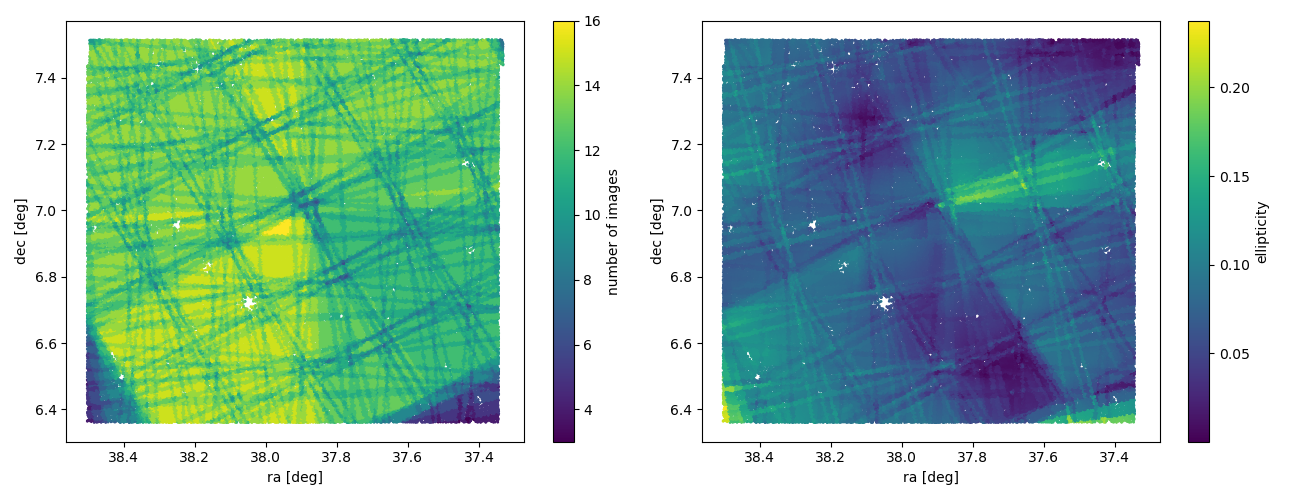
\includegraphics[width=\textwidth]{Figures/psf_ellipticity_visits.png}
\caption{\emph{Left}: number of images used in the coadded data in the field of A360. \emph{Right}: modulus of the PSF ellipticity in the field. The dithering pattern appears clearly in both figures.\label{fig:dither}}
\end{figure}

For each band, the object table also includes the second moments of the object surface brightness $I_{xx,xy,yy}$ and second moments of the PSF model $I_{xx,xy,yy}^{\rm PSF}\,$, both measured using HSM \citep{2003MNRAS.343..459H, 2005MNRAS.361.1287M, 2018MNRAS.481.3170M}. A flag in the catalog identifies stars that have been used by Piff to build the PSF model; these are termed PSF stars. Additionally, a set of reserved stars (selected with the same criteria as PSF stars, but not used in the fit) are flagged in the catalog for the purpose of PSF testing (e.g., \citealp{2025OJAp....8E..26S}). 
With that selection, there are 1977 PSF stars and 229 reserved stars at our disposal to run the PSF diagnostics tests below. 

\paragraph*{Software} This work was run on the Rubin Science Plateform Notebook Aspect at USDF. The A360-related notebooks, including the ones developed for this work are publicly available in a GitHub repository\footnote{\url{https://github.com/lsst-sitcom/comcam_clusters}}.
The figures in this note have been produced using the following:
\begin{itemize}
\item \code{repo = '/repo/dp1'}
\item \code {collection = 'LSSTComCam/runs/DRP/DP1/v29\_0\_0/DM-50260'}
\item Science pipeline version: \code{Weekly 2025\_17}
\end{itemize}



\section{PSF properties and diagnostics}

From the second moment matrix expressed in the (x,y) frame of the tracts, we define:
\begin{itemize}
\item The trace 
\begin{equation}
T = I_{xx} + I_{yy}
\end{equation}

\item The ellipticities e1, e2
\begin{eqnarray}
  e_1 &=& (I_{xx} - I_{yy})/T \\
  e_2 &=& 2 I_{xy} / T
\end{eqnarray}

\item The modulus of the ellipticity $e$ and the orientation $\theta$ of the major axis of the ellipse with respect to the x axis, given by
\begin{equation} 
e = \sqrt{e_1^2 + e_2^2}
\label{eq:modulus}
\end{equation}
\begin{equation}
\theta = 0.5 \times \arctan(e_2/e_1)
\label{eq:theta}
\end{equation}
\end{itemize}


From these, we compute the residuals between the measurements for the set of PSF (or reserved) stars and that of the PSF model at their locations.  Namely,
\begin{eqnarray}
\delta e_1 &=& e_1^{\rm meas} - e_1^{\rm model}, \, \delta e_2 = e_2^{\rm meas} - e_2^{\rm model}\\
\delta T &=& T^{\rm meas} - T^{\rm model} 
\end{eqnarray}

Before looking into the residuals in the next section, the right panel in Figure~\ref{fig:dither} displays the modulus of the PSF model ellipticity in the field. While the mean ellipticity across the field is ~0.07, there are several areas where the PSF ellipticity reaches significant values. This could be investigated further by checking the PSF at the individual visit level; this goes however beyond the scope of this technote which aims at checking, in the next section, whether the PSF modeling is sufficient for the purpose of measuring a lensing profile around A360.
  


\subsection{PSF residuals - distributions and whisker plots}
To assess the performance of the PSF model, a first test consists in comparing the normalized distribution of the residuals defined above, for the PSF and reserved stars, to check for a possible overfitting of the PSF model \citep{2025OJAp....8E..26S}. As can be seen in Figure~\ref{fig:residual_distrib} (left and middle panels), the ellipticity residuals peak around zero and extend to $\sim 0.02$. The right panel shows the relative residuals of the trace, peaked around zero and not exceeding beyond $\sim 5 \%$. The residuals obtained from the PSF stars and reserved stars behave similarly, not indicating any overfitting of the PSF model.

\begin{figure}
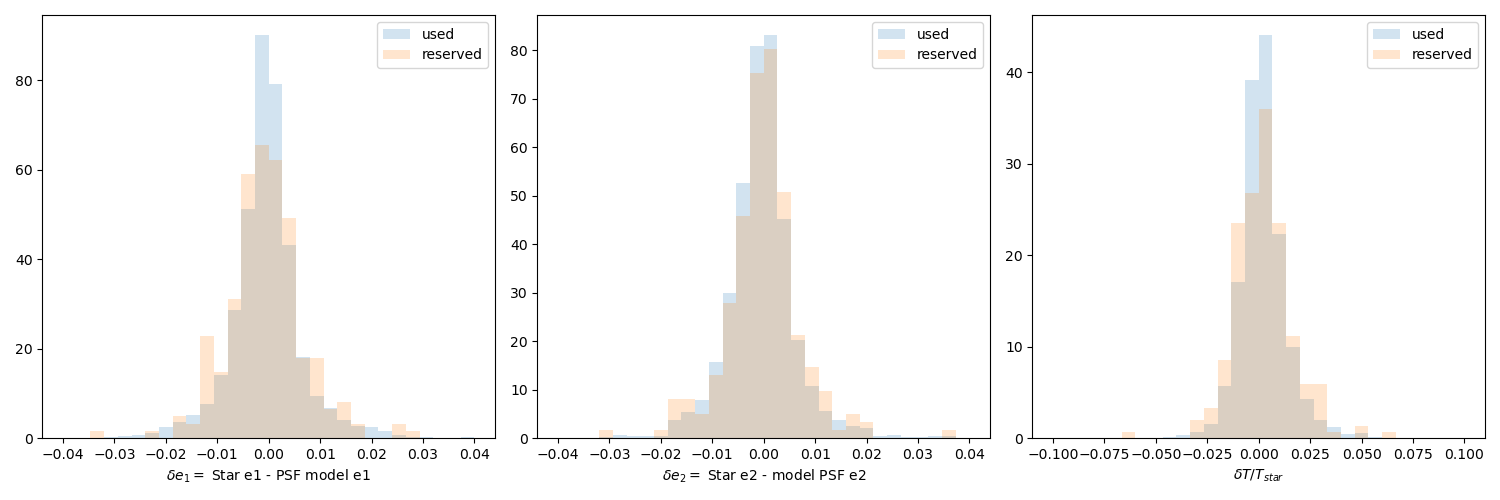
\includegraphics[width=\textwidth]{Figures/residual_histograms.png}
\caption{Normalised distributions of the ellipticity residuals $\delta e_1$ (left), $\delta e_2$ (right), and of the relative residuals $\delta T/T$ (right). The distributions are shown for the PSF (blue) and reserved (orange) sets of stars. \label{fig:residual_distrib}}
\end{figure}


Figure~\ref{fig:whiskers} shows the variation of the PSF ellipticity and residuals across the field of A360. Each whisker is oriented according the direction of the ellipse major axis ($\theta$, Eq.(\ref{eq:theta})) and its length is proportional to the ellipticity modulus ($e$, Eq.(\ref{eq:modulus})); this is done for the PSF stars (top row) or reserved stars (bottom row). The left panel corresponds the measurements on the star themselves, the middle panel shows the corresponding PSF model, and the residuals are displayed in the right panel. A reference whisker is given for an ellipticity $e = 0.1$. The circle corresponds to a $0.5^\circ$  field around the cluster’s BCG, i.e., corresponding to $\sim 6$~Mpc at the cluster's redshift (roughly the field we aim the WL measurements at). Looking at the residuals (right panel), we conclude that the PSF model perfoms satisfactorily, in particular as it is successful at correcting the coherent ellipticity patterns seen across the field.


\begin{figure}
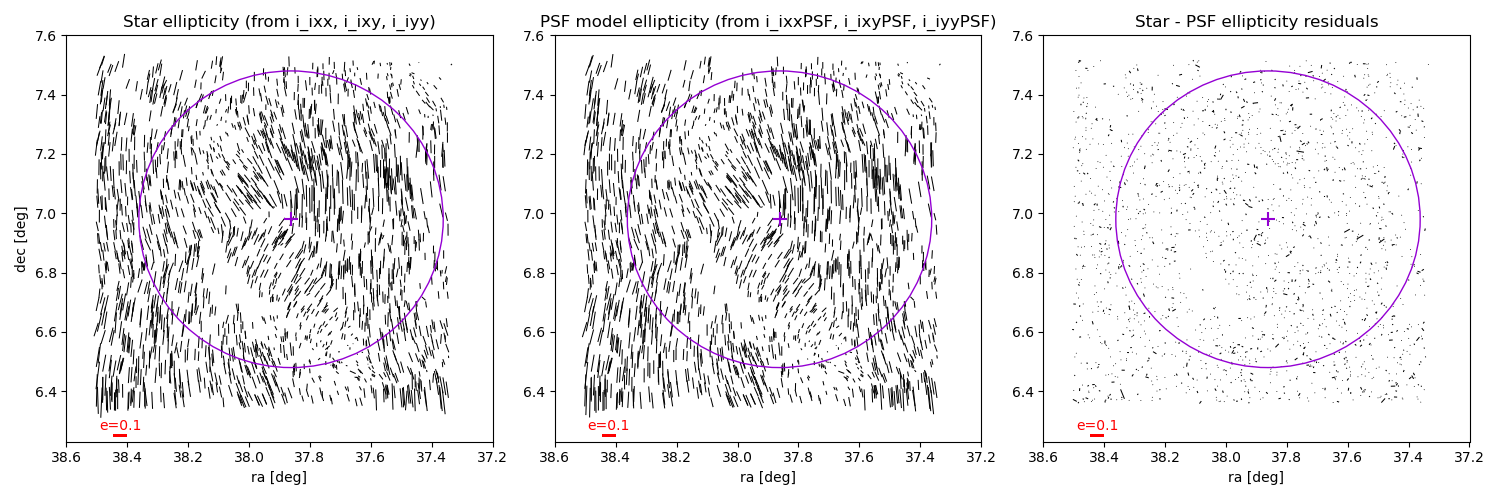
\includegraphics[width=\textwidth]{Figures/whiskers_used.png}
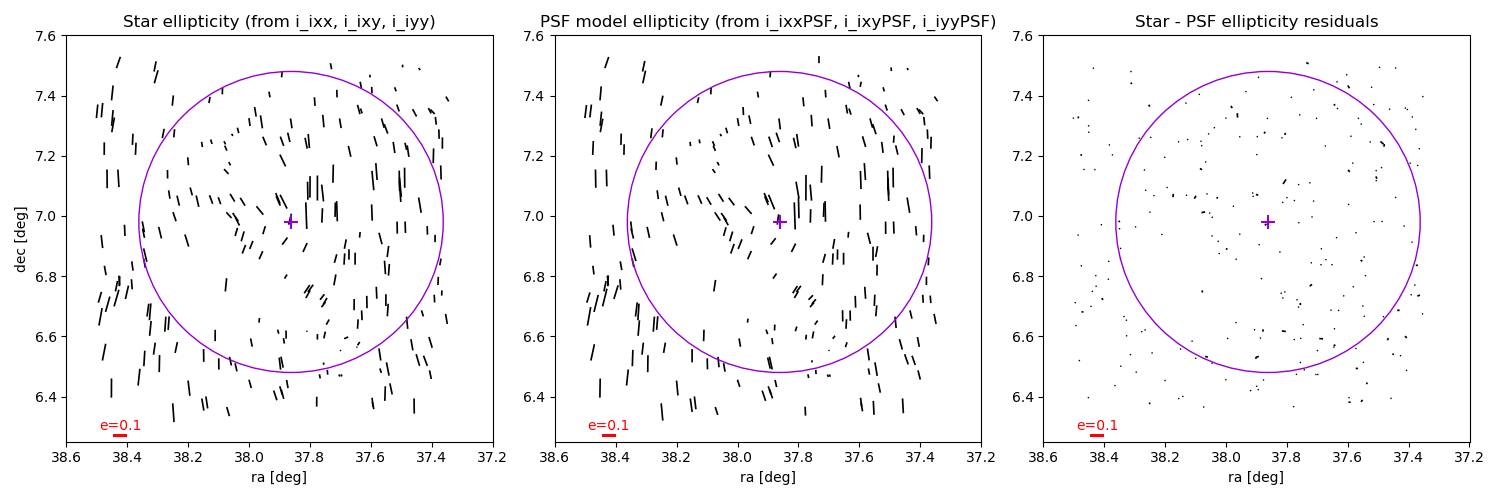
\includegraphics[width=\textwidth]{Figures/whiskers_reserved.png}
\caption{Whikser plots for the PSF (top) and reserved stars (bottom) obtained for the measurements (left), PSF model (middle) and the residuals (right). The size of the whiskers is proportional to the ellipticity modulus and the orientation gives the direction of the major axis of the ellipse. \label{fig:whiskers}}
\end{figure}

\subsection{PSF residuals - tangential shear profile}

An important diagnostic for cluster weak lensing is to evaluate the contribution of the PSF residuals to the tangential shear signal. To do so, we compute the tangential component of the residuals $\delta e_t$ as 
\begin{equation}
\delta e_t = - \delta e_1  \cos(2 \phi) - \delta e_2  \sin(2 \phi),
\end{equation}
where $\phi$ is the position angle at the location of the computed residuals.

Figure~{\ref{fig:res_profile}} shows the corresponding binned radial profile as a function of the angular separation to the cluster center. The profile for PSF stars shows smaller error bars because of the larger number compared to the reserved set of the stars. The profiles are generally consistent with zero, but for a few radial bins where the amplitude is in any case more than an order of magnitude lower than the typical expected signal for the cluster with mass of A360 (see Section~\ref{sec:shear_profile}). 

\begin{figure}
\centering
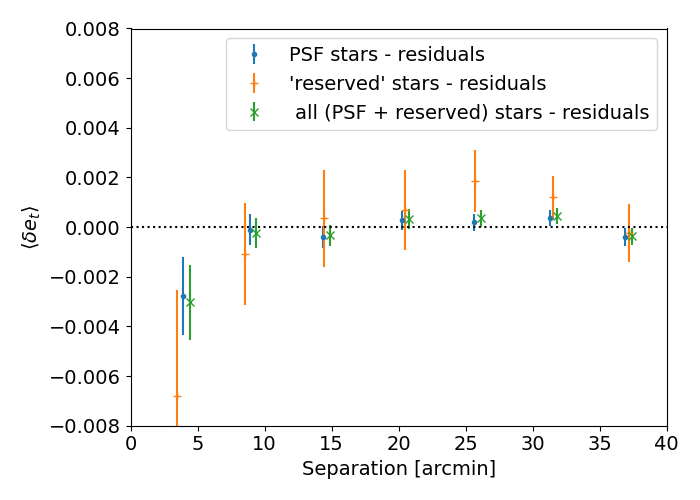
\includegraphics[width=0.7\textwidth]{Figures/residual_tan_profile_CLMM.png}
\caption{Binned tangential profile of the ellipticity residuals for the PSF stars (blue circle), for the reserved stars (orange plus sign marker), and for both sets together (green cross).\label{fig:res_profile}}
\end{figure}


\subsection{PSF rho-statistics}
The $\rho$-statistics \citep{2010MNRAS.404..350R, 2016MNRAS.460.2245J} are a set of two-point correlation functions involving PSF ellipticity and size residuals. They quantify spatial correlation errors in PSF modeling and contributions from PSF leakage. We used the LSST Science Pipelines \code{analysis\_tools}\footnote{\url{https://pipelines.lsst.io/v/daily/modules/lsst.analysis.tools}} implementation to compute the $\rho$-statistics, which internally relies on the TreeCorr software package \citep{2015ascl.soft08007J} for the correlation function calculations. The definitions of the $\rho$-statistics as calculated by \code{analysis\_tools} are documented in the LSST pipelines and include those originally introduced by \citet{2010MNRAS.404..350R, 2016MNRAS.460.2245J}, as well as an additional one defined in the context of cluster analysis by \citet{2015MNRAS.449.2219M}.

We used the set of reserved stars to calculate the rho statistics in the $i$-band, and display the results in Figure~\ref{fig:rho_stat}.

\begin{figure}
\centering
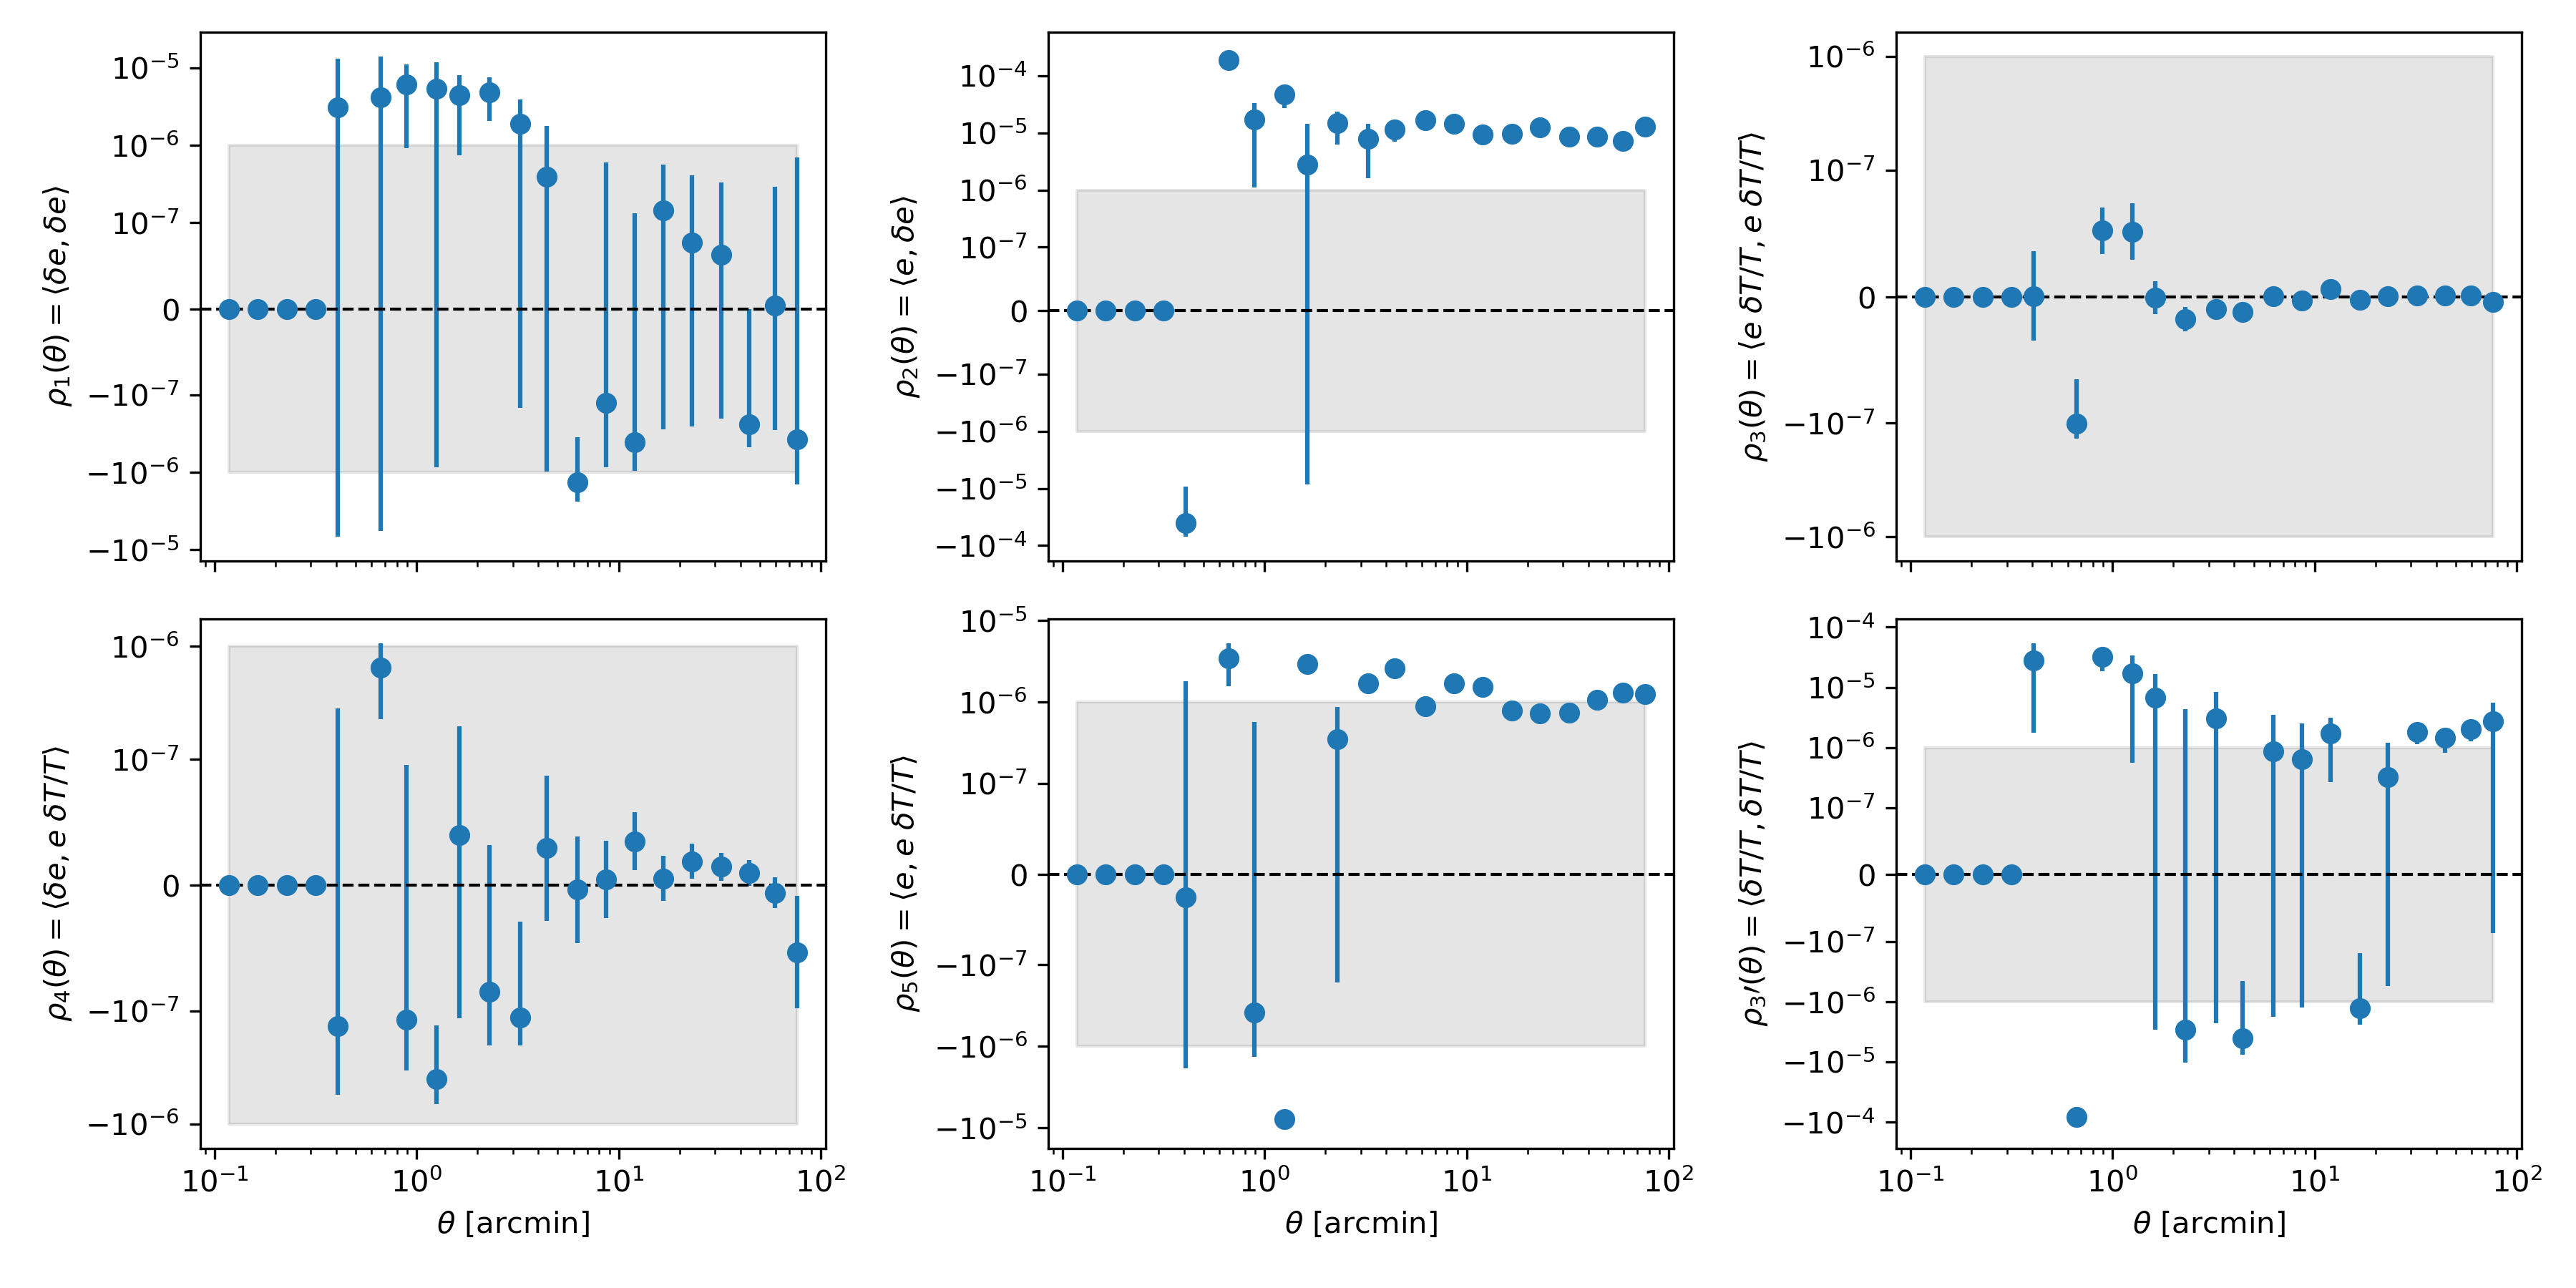
\includegraphics[width=\textwidth]{Figures/rho_stat.png}
\caption{The various $\rho$-statistics correlations as a function of separation, as produced by the Rubin \code{AnalysisTools} software. The grey band indicate the $\pm 10^{-6}$ level in all panels.\label{fig:rho_stat}}
\end{figure}


For this cluster, the size scale is a few arcminutes. In the $\rho_2$ plot, we see that the PSF shape modeling bias (square root of $\rho_2$) is $\lesssim 10^{-3}$ at the cluster length scale that we are interested in. We note that the typical shear is $\sim 3\times10^{-2}$ (see Figure~\ref{fig:shear_profile}). Thus, the PSF modeling bias is $\sim <0.3/3=10$, i.e. one order of magnitude lower than the shear. This is consistent with our previous conclusion, which means the bias is sufficiently small in our shear measurement.


\section{HSM tangential and cross shear profile around A360 from simple color-cut selection}
\label{sec:shear_profile}

From the tests above, it appears that the PSF modeling in the A360 field is sufficiently accurate not to hinder a first attempt at measuring the tangential and cross shear profiles around that cluster. The cross shear profile is a particularly useful null test to highlight remaining systematics effects. We therefore proceed to do so, using the \code{shapeHSM} ellipticities readily available in the object table (other shape measurements methods, such as \code{Metadetect} or \code{Anacal} will be explored elsewhere; see \citet{SITCOMTN-162} for the \code{Metadetect} analysis). 

For this preliminary work, we use a visual inspection of the $r-i$ versus $r$ color-magnitude diagram to select and remove red sequence galaxies from the sample. Source selection in other colors and using photoz is explored more thoroughly in \citet{SITCOMTN-163}. 
Given that the ComCam field of A360 reaches roughly similar depth as HSC Y1 and uses a similar pipeline, we use the HSC Y1 lensing quality cuts and shear calibration procedure\footnote{The script to applied the calibration is available at \url{https://github.com/PrincetonUniversity/hsc-y1-shear-calib}. It was slightly adapted to use the column names from the object table.} \citep{2018MNRAS.481.3170M} to convert the e1 and e2 ellipticities into g1 and g2 shear estimates. Once the calibration has been applied, we use the DESC CLMM package \citep{2021MNRAS.508.6092A} to compute the tangential and cross reduced shear radial profiles, displayed in Figure~\ref{fig:shear_profile}. The physical distance on the x-axis is obtained from the angular separation assuming a default cosmology, and ranges from 0.4 Mpc to 6 Mpc (to match the circular 0.5 deg field highlighted in the PSF diagnostic plots at the upper end, and to avoid the cluster inner regions known to be affected by other sources of biases such as miscentering and sample contamination). 

\begin{figure}
\centering
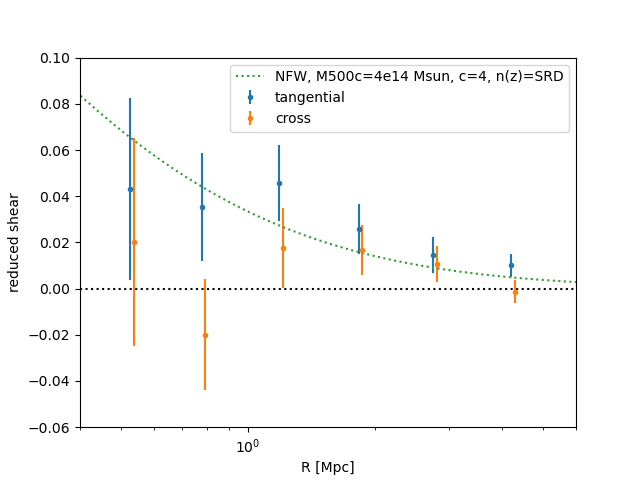
\includegraphics[width=0.7\textwidth]{Figures/shear_profile.png}
\caption{Binned tangential (blue) and cross (orange) reduced shear profile around A360. The green dashed line corresponds shows the expected signal for a NFW halo of mass similar to that of A360, a concentration $c=4$, and assumes the redshift distribution $n(z)$ of the DESC Science Requirement document. \label{fig:shear_profile}}
\end{figure}

First, the cross shear signal, in orange, scatters around zero, indicating that no significant remaining systematics exists in the measurement. Second, we see a positive tangential shear signal, increasing towards the inner regions as expected. While this analysis is too preliminary to conclude on the robustness of the measured signal, we overplot in dashed green the expected signal from a NFW halo with the mass of A360, an assumed concentration c=4, and a source redshift distribution matching that of the DESC Science Requirements Document \citep{2018arXiv180901669T}; the actual photometric distribution in that field will be studied elsewhere. We see that the measured tangential shear is in the ballpark of what one could expect with these simplifying assumptions, although more work is required to robustify this result.


\section{Conclusion}
We have checked the PSF model in the field of the galaxy cluster A360, which was observed in the low ecliptic latitude field of the Rubin 2024 ComCam campaign. While the PSF ellipticity reaches values as high as >~0.2 in the coadd data, we find that the model is able to capture and correct the PSF, at a level sufficient not to impact the measurement of the shear profile around A360. 


\appendix
% Include all the relevant bib files.
% https://lsst-texmf.lsst.io/lsstdoc.html#bibliographies
\section{References} \label{sec:bib}
\renewcommand{\refname}{} % Suppress default Bibliography section
\bibliography{local,lsst,lsst-dm,refs_ads,refs,books}

% Make sure lsst-texmf/bin/generateAcronyms.py is in your path
\section{Acronyms} \label{sec:acronyms}
\addtocounter{table}{-1}
\begin{longtable}{p{0.145\textwidth}p{0.8\textwidth}}\hline
\textbf{Acronym} & \textbf{Description}  \\\hline

DESC & Dark Energy Science Collaboration \\\hline
DM & Data Management \\\hline
DMTN & DM Technical Note \\\hline
DP1 & Data Preview 1 \\\hline
DRP & Data Release Processing \\\hline
HSC & Hyper Suprime-Cam \\\hline
HSM & Hierarchical Storage Management \\\hline
LSST & Legacy Survey of Space and Time (formerly Large Synoptic Survey Telescope) \\\hline
LSSTComCam & Rubin Commissioning Camera \\\hline
PSF & Point Spread Function \\\hline
RTN & Rubin Technical Note \\\hline
SE & System Engineering \\\hline
SNR & Signal to Noise Ratio \\\hline
SV & Science Validation \\\hline
TBC & To Be Confirmed \\\hline
USDF & United States Data Facility \\\hline
WL & Weak gravitational Lens cosmic shear \\\hline
\end{longtable}

% If you want glossary uncomment below -- comment out the two lines above
%\printglossaries





\end{document}
